\documentclass{article}

\usepackage[nonatbib,preprint]{nips_2018}

\usepackage[T1]{fontenc}    % use 8-bit T1 fonts
\usepackage[utf8]{inputenc} % allow utf-8 input
\usepackage{hyperref}       % hyperlinks
\usepackage{url}            % simple URL typesetting
\usepackage{booktabs}       % professional-quality tables
\usepackage{amsfonts}       % blackboard math symbols
\usepackage{nicefrac}       % compact symbols for 1/2, etc.
\usepackage{microtype}      % microtypography
\usepackage{optidef}
\usepackage[]{graphicx}
\usepackage{stmaryrd}
\usepackage{mathtools}
\usepackage{algpseudocode}
\usepackage{algorithm}
\usepackage{listings}
\usepackage[outdir=../plots/]{epstopdf}

\usepackage{color}
 
\definecolor{codegreen}{rgb}{0,0.6,0}
\definecolor{codegray}{rgb}{0.5,0.5,0.5}
\definecolor{codepurple}{rgb}{0.58,0,0.82}

\lstdefinestyle{mystyle}{
  commentstyle=\color{codegreen},
  keywordstyle=\color{magenta},
  numberstyle=\tiny\color{codegray},
  stringstyle=\color{codepurple},
  basicstyle=\footnotesize\tt,
  breakatwhitespace=false,         
  breaklines=true,                 
  captionpos=b,                    
  keepspaces=true,                 
  numbers=left,                    
  numbersep=5pt,                  
  showspaces=false,                
  showstringspaces=false,
  showtabs=false,                  
  tabsize=2
}

\lstset{style=mystyle}

\usepackage[
  backend=biber,
  style=nature,
  sorting=ynt
]{biblatex}
\addbibresource{main.bib}


\newcommand{\RR}{\mathbb{R}}
\DeclarePairedDelimiter{\norm}{\|}{\|}
\DeclarePairedDelimiter{\ip}{\langle}{\rangle}
\DeclarePairedDelimiter{\set}{\{}{\}}
\DeclarePairedDelimiter{\ex}{\mathbb{E}[}{]}
\newcommand{\inv}{{}^{-1}}
\newcommand{\trans}{{}^{\top}}


\title{A Stochastic Quasi-Newton Optimizer for TensorFlow}


\author{
  Jason Chen \\
  Department of Computer Science \\
  Stony Brook University \\
  Stony Brook, NY 11790 \\
  \texttt{hungrchen@cs.stonybrook.edu} \\
  \And
  David Kraemer \\
  Department of Applied Mathematics\\
  Stony Brook University \\
  Stony Brook, NY 11790 \\
  \texttt{davidkraemer@stonybrook.edu}
}

\date{May 6, 2018}


\begin{document}


\maketitle


\begin{abstract}
  We do some shit and it doesn't work.
\end{abstract}


\section{Introduction}


%\begin{enumerate}
%  \item Introduce problem that SdLBFGS solves.
%  \item TensorFlow current state of the art.
%  \item Problems with the TensorFlow state.
%  \item Overview of paper.
%\end{enumerate}


Limited memory variations of classical second-order minimization algorithms can
prove highly attractive in applications with high-dimensional problems or when
the cost of each iteration step is prohibitive under these classical
formulations.  Specifically, the canonical second-order technique, Newton's
method, involves explicit computation of the Hessian matrix of the objective
function, whose time complexity grows with the square of the parameter
dimension. Even with BFGS, which seeks to reduce the direct computational
difficulty of exactly constructing the Hessian itself, encounters similar
difficulties of scale. The limited memory approach is to bound this overall cost
and ensure that approximate Hessians can be computed on existing hardware.

We implement a variant of stochastic second-order algorithm as described by
Wang, Ma, Goldfarb, and Liu \cite{sdlbfgs} for application in the
\texttt{TensorFlow} library \cite{tensorflow}.  \texttt{TensorFlow} is a
framework for graph-based computation models. Its primary use within the
statistical learning community is in neural networks, which can be readily
implemented by the library. After the model is constructed, the actual training
is performed by an \texttt{Optimizer} object. In this setting, the
\texttt{Optimizer} is presented with a partially observable objective function
and gradient from which to perform optimization. Some typical \texttt{Optimizer}
subclasses which are available in the Python API include
an \texttt{GradientDescentOptimizer}\footnote{%
  See
  \href{https://github.com/tensorflow/tensorflow/blob/master/tensorflow/python/training/gradient_descent.py}{source.}
}% 
and an \texttt{AdagradOptimizer}\footnote{%
  See \href{https://github.com/tensorflow/tensorflow/blob/master/tensorflow/python/training/adagrad.py}{source.}
}%

The presently available optimization algorithms implemented in the Python
library are either first or zeroeth-order methods, requiring access to either
the objective function or its gradient. The conspicuous absence of second-order
methods, such as Newton or quasi-Newton algorithms, has been a subject of much
discussion inside the \texttt{TensorFlow} community\footnote{%
  The primary discussion has occurred surrounding
  \href{https://github.com/tensorflow/tensorflow/issues/446}{Issue \#446}, in
  which contributors have noted that the current infrastructure for developing
  second-order methods is lacking and any implementation would require
  considerable re-inventing the wheel.
.}

Following the suggestions of the community discussion, we present an
implementation of Stochastic damped limited memory BFGS (SdLBFGS) for
\texttt{TensorFlow} through the use of an \texttt{ExternalOptimizerInterface}.
Presently used to wrap existing minimization routines implemented by outside
libraries such as \texttt{SciPy}, it serves as a simple way to engage with the
\texttt{TensorFlow} internals while avoiding a deep dive into its architecture.

Our work proceeds as follows. Section 2 reviews the problem proposed in Wang et
al and gives an explicit formulation of SdLBFGS according to their paper. We
identify small modifications made to the core pseudocode and explain their
necessity. Section 3 describes our SdLBFGS implementation and how it interfaces
with \texttt{TensorFlow}. Section 4 shows preliminary experimental results on
the correctness of our implementation on simple problems. Importantly, we report
that our present implementation is incapable of giving meaningful progress on
training practical models on common datasets. In Section 5, we discuss the
implications of this negative result on future development and specify areas in
which our project may be continued and improved.

Source code for this project can be found at
\url{https://github.com/DavidNKraemer/cse592-project}. Documentation, cruft
removal, and user interface improvements are currently evolving.

\section{Review of theory}


\begin{enumerate}
  \item Review main results of the Wang, Ma, Goldfarb, Liu paper
    \cite{sdlbfgs}
  \item State the SdLBFGS algortihm.
  \item Mention some details about how the algorithm translates to code.
\end{enumerate}


The SdLBFGS algorithm is proposed by Wang, Ma, Goldfarb, and Liu \cite{sdlbfgs}
for solving nonconvex stochastic optimization problems. In particular, it solves
\begin{mini}
  {x \in \RR^n}{f(x) = \ex{F(x, \xi)}}{}{} 
  \label{prb:mini}
\end{mini}
for $F \in C^1(\RR^n \times \RR^d)$ and $\xi \in \RR^d$ is a random variable
with cumulative distribution function $P$. Here $\ex{\cdot}$ denotes the
mathematical expectation. In general $F$ need not be convex.

The function $F$ is readily interpreted in the context of supervised statistical
learning.  Given a corpus $\Xi$ of data, we put a distribution on $\Xi$ which
reflects a sampling regime for a training set. The object of the learning
process is, then, to the model parameter $x \in \RR^n$ which minimizes $F$
\emph{in expectation} with respect to the training set. Provided that the
sampling maintains some resemblance to the overall corpus, this gives a useful
approximate parameter for the whole corpus.

The SdLBFGS algorithm emerges from two concurrent optimization techniques.
First, it follows in the tradition of approximate second-order algorithms which
seek to perform a version of Newton's method while avoiding the computation of
the Hessian $\nabla^2 f(x)$ explicitly. The classical BFGS approach is the
canoncal quasi-Newton method. Second, it follows the development of stochastic
algorithms which seek to randomly sample the components of the gradient $\nabla
f(x)$ so that the essential convergence properties hold in expectation. In this
sense it succeeds Stochastic Gradient Descent, among other canonical methods of
this class. The limited memory constraint has antecedents in both streams of
optimization techniques.

Wang et al. \cite{sdlbfgs} assume that Problem (\ref{prb:mini}) satisfies the
following assumptions:
\begin{enumerate}
  \item There is a real lower bound for $f$. That is, $\inf_{x \in \RR^n} f(x) >
    -\infty$.
  \item The gradient $\nabla f$ is Lipschitz continuous. That is, there exists
    $L > 0$ such that 
    \begin{equation*}
      \norm{\nabla f(x) - \nabla f(y)} \leq L \norm{x - y}
    \end{equation*}
    for all $x,y \in \RR^n$. Moreover, $\nabla_{xx} F(x, \xi)$ exists and is
    continuous, and there exists $\kappa > 0$ with $\norm{\nabla^2_{xx} F(x,
    \varepsilon)} \leq \kappa$ for any $x, \xi$.
  \item The sampling regime is unbiased. That is, for the $k$th iterate the
    following hold:
    \begin{align*}
      \ex{g(x_k, \xi_k)}_{\xi_k} &= \nabla f(x_k), \\
      \ex{\norm{g(x_k, \xi_k) - \nabla f(x_k)}^2}_{\xi_k} &\leq \sigma^2,
    \end{align*}
    where $g(x, \xi_k) = \nabla F(x, \xi_k)$ and $\sigma^2$ is the noise level
    of estimating $g(x, \xi_k)$. 
\end{enumerate}

For a convex function, $\nabla^2 f(x)$ is always positive semidefinite (see Boyd
and Vandenberghe \S 3.1.4 \cite{boyd}), but this need not be the case in for
nonconvex functions. The work in Wang et al.  \cite{sdlbfgs} shows how the BFGS
approximate Hessian may be tweaked to ensure that positive semidefiniteness is
preserved even in nonconvex cases. The overall stochastic quasi-Newton method is
described in Algorithm \ref{alg:sqn}, while the detailed implementation of
SdLBFGS is given in Algorithm \ref{alg:sdlbfgs}.

We note that the formulation of Algorithm \ref{alg:sdlbfgs} differs slightly
from Wang et al. In the original paper, the use of $\textrm{mem}$ in the section
corresponding to lines 15 and 16 of Algorithm \ref{alg:sdlbfgs} is replaced by
$p$. This leads to the difficulty that if $p$ indicates memory \emph{capacity}
rather than simply the current amount of data in memory, the indices can become
negative early in the iteration. Specifically, when $k < p$ in the original
paper the algorithm has undefined behavior. We clarify this ambiguity in the
following way: in our implementation, $p$ indicates the total memory capacity of
the procedure, regardless of the total amount of memory presently in use. The
quantity $\textrm{mem}$ replaces $p$ in the SdLBFGS update step so as to prevent
array index out of bounds errors when $k$ is small (i.e., $k < p$), but both our
implementation and the original paper's exhibit the same behavior whenever $k >
p$.

\begin{algorithm}
  \begin{algorithmic}[1]
    \Function{SQN}{$x_1, \ip{m_k}_{k=1}^{\infty},
    \ip{\alpha_k}_{k=1}^{\infty}, p$}
    \State{$\textrm{data} \leftarrow \textit{nil}()$}
    \For {$k = 1, 2, \dots$}
    \State{$g_k \leftarrow \frac{1}{m_k} \sum_{i=1}^{m_k} g(x_k,
    \varepsilon_{k,i})$} 
    \State{$\Delta x_k, s_{k-1}, \bar{y}_{k-1}, \rho_{k-1} \leftarrow
    \textsc{SdLBFGS}(g_k, {}^*(\textrm{data}\trans))$} \Comment{Tuple unpacking}
    \State{$x_{k+1} \leftarrow x_k - \alpha_k \Delta x_k$}
    \State{$\textit{append}(\textrm{data}, (s_{k-1}, \bar{y}_{k-1}, \rho_{k-1}))$}
    \If{$k > p$}
    \State{$\textit{pop}(\textrm{data})$}
    \EndIf
    \EndFor
    \EndFunction
  \end{algorithmic}
  \label{alg:sqn}
  \caption{%
    The high level stochastic quasi-Newton minimization algorithm. Given an
    initial point $x_1 \in \RR^n$, batch sizes $\ip{m_k}$, step sizes
    $\ip{\alpha_k}$, and a maximum memory capacity $p$, perform BFGS with the
    stochastic dampened direction update.
  }
\end{algorithm}

\begin{algorithm}
  \begin{algorithmic}[1]
    \Function{SdLBFGS}{$g_{k-1}, \ip{s_{j}}_{j=k-p}^{k-2},
    \ip{\bar{y}_{j}}_{j=k-p}^{k-2}, \ip{\rho_{j}}_{j=k-p}^{k-2}$}
    \State{$\textrm{mem} \leftarrow \textit{min}(p, k-1)$}
    \State{$s_{k-1} \leftarrow x_k - x_{k-1}$}
    \State{$y_{k-1} \leftarrow \frac{1}{m_{k-1}}\sum_{i=1}^{m_{k-1}}[g(x_k,
    \xi_{k-1,i}) - g(x_{k-1}, \xi_{k-1,i})]$}
    \State{$\gamma_k \leftarrow \textit{max}\left( \frac{y_{k-1}\trans
    y_{k-1}}{s\trans_{k-1}y_{k-1}}, \delta \right) \geq \delta$}
    \State{%
      $\theta \leftarrow
      \textit{max}\left( 
        \frac{3}{4} \frac{\gamma_{k}\inv s_{k-1}\trans
        s_{k-1}}{\gamma_k\inv s_{k-1}\trans s_{k-1} - s_{k-1}\trans y_{k-1}}, 1
      \right)
    $}
    \Comment{$\theta$ preserves positive semidefiniteness.}
    \State{$\bar{y}_{k-1} \leftarrow \theta y_{k-1} + (1 -\theta \gamma_{k}\inv s_{k-1})$}
    \State{$\rho_{k-1} \leftarrow (s_{k-1}\trans \bar{y}_{k-1})\inv$}
    \For{$i =0 , \dots, \textrm{mem}-1$}
    \State{$\mu_i \leftarrow \rho_{k-i-1} u_i\trans s_{k-i-1}$} 
    \State{$u_{i+1} \leftarrow u_i - \mu_i \bar{y}_{k-i-1}$}
    \EndFor
    \State{$v_0 \leftarrow \gamma_k\inv u_{\textrm{mem}}$}
    \For{$i =0 , \dots, \textrm{mem}-1$}
    \State{$\nu_i \leftarrow \rho_{k-\textrm{mem}+i} v_i\trans
    \bar{y}_{k-\textrm{mem}+i}$}
    \State{$v_{i+1} \leftarrow v_i + (\mu_{\textrm{mem}-i-1} - \nu_i)s_{k-\textrm{mem}+i} $}
    \EndFor
    \State{\Return{$v_p, s_{k-1}, \bar{y}_{k-1}, \rho_{k-1}$}}
    \EndFunction
  \end{algorithmic}
  \caption{%
    The SdLBFGS update step. The resulting output is $H_k g_k = v_p$,
    where $H_k$ is the approximation of the $k$th iterate Hessian and $g_k$ is the
    approximation of the $k$th iterate gradient. Note that the computation of $H_k$
    is implicit, preventing additional storage requirements.
  }
  \label{alg:sdlbfgs}
\end{algorithm}




\section{Implementation}


% \begin{enumerate}
%   \item Describe how TensorFlow algorithms are usually implemented.
%   \item Contrast with our implementation of SdLBFGS.
%   \item Explain some implementation issues.
% \end{enumerate}

Our optimization object, \texttt{SQNOptimizer}, is implemented using
\texttt{NumPy} \cite{numpy} with \texttt{ndarray} objects serving as the primary
data structures for the numerical computations in Algorithm \ref{alg:sdlbfgs}.
It inherits the features of the \texttt{ExternalOptimizerInterface}, which
packages the objective function and its gradients from the network model in use
and presents it in a \texttt{NumPy}-interoperable format. 

The general framework for using built-in \texttt{Optimizer} objects follows the
structure presented in Figure \ref{fig:typical}.
\begin{figure}[h]
  \begin{lstlisting}[language=Python]
# ... setup
optimizer = Optimizer(**kwargs).minimize(objective_function)
# ... setup
with tf.Session() as session:
    # ... training setup
    optimizer.run(**training_kwargs)
  \end{lstlisting}
  \caption{The typical workflow for using built-in \texttt{Optimizer} objects in
    a statistical learning setting. Here the \texttt{optimizer} is an operation
    which is configured to minimize the objective function. The actual
  minimization occurs inside of the session block.}
  \label{fig:typical}
\end{figure}
The initialization of line 2 indicates that \texttt{optimizer} is a minimization
operation, rather than the result of a minimization. By contrast, for subclasses
of an \texttt{ExternalOptimizerInterface}, this structure is replaced by the
workflow in Figure \ref{fig:external}.
\begin{figure}[h]
  \begin{lstlisting}[language=Python]
# ... setup
optimizer = ExternalOptimizer(objective_function, **kwargs)
# ... setup
with tf.Session() as session:
    # ... training setup
    optimizer.minimize(session, **training_kwargs)
  \end{lstlisting}
  \caption{%
    The workflow for using objects of 
  \texttt{ExternalOptimizerInterface} subclasses, such as the implementation of
  \texttt{SQNOptimizer}. Here the \texttt{optimizer} itself is the minimizer while
  the \texttt{minimize} method actually performs estimation of the minimal
  objective function value.  }
  \label{fig:external}
\end{figure}

Now, the \texttt{minimize} method returns the \emph{result} of a minimization
rather than a minimization operation. As \texttt{SQNOptimizer} inherits this
functionality, the second workflow is required. 

\section{Empirical results}


\begin{enumerate}
  \item Results on simple optimization problems. 
  \item Results on potentially more difficult optimization problems.
  \item Lack of results on MNIST with TensorFlow.
\end{enumerate}



\begin{figure}[h]
  \centering
  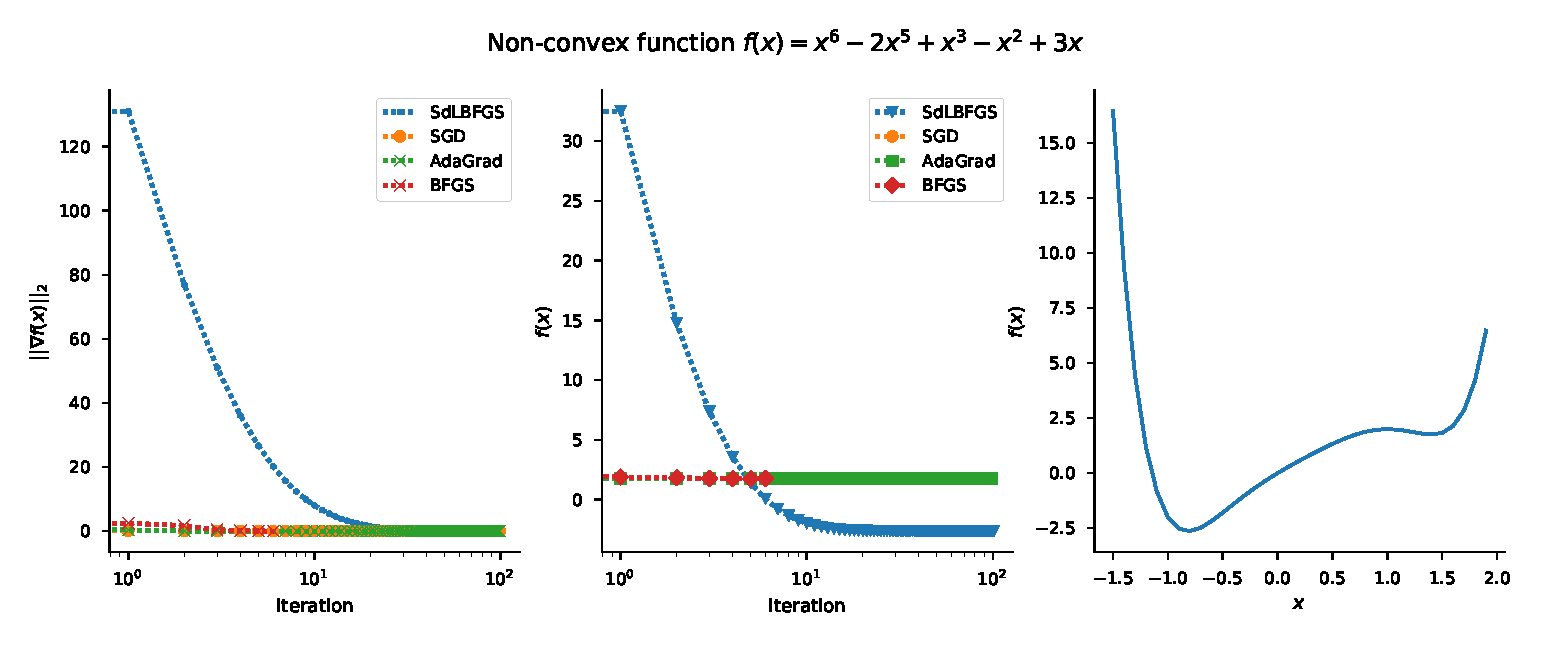
\includegraphics[width=\textwidth]{../plots/nonconvex_results}
  \caption{
    SdLBFGS compared with traditional BFGS together with AdaGrad and Stochastic
    Gradient Descent on the problem $f(x) = x^6 - 2x^5 + x^3 - x^2 + 3x$, shown
    on the right. Each algorithm is initialized near the local minimum at around
    $x = 1.6$. We see that SGD, AdaGrad, and BFGS quickly converge to the local
    minimum, whereas SdLBFGS converges to the global minimum at around $x =
    -0.8$ more slowly.
  }
  \label{fig:convex-linear-system}
\end{figure}

\begin{figure}[h]
  \centering
  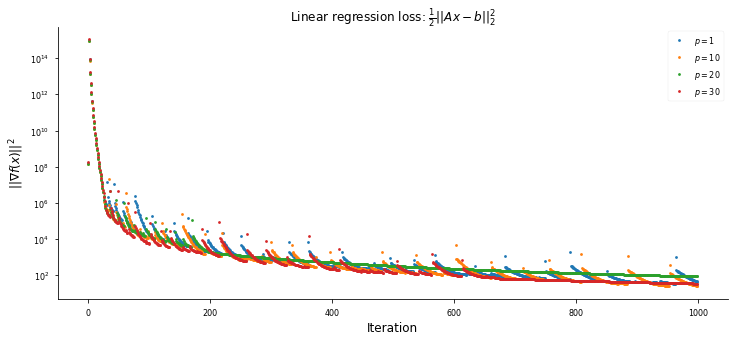
\includegraphics[width=\textwidth]{../plots/linear_system_loss}
  \caption{
    SdLBFGS performance on the solving the overdetermined linear system
    $Ax = b$ with $A \in \RR^{50 \times 100}$ with convex smooth loss function
    $\norm{Ax-b}_2^2$. We sweep different memory capacity values $p \in
    \set{1,10,20,30}$ and observe that convergence is approximately equivalent
    between configurations.
  }
  \label{fig:convex-linear-system}
\end{figure}


\section{Discussion}


\begin{enumerate}
  \item Explaining why the basic project --- implementing a useful practical
    TensorFlow optimzier --- failed.
  \item Takeaways from the results.
  \item Future work.
\end{enumerate}


\printbibliography[heading=bibintoc]


\end{document}
